\documentclass[12pt]{article}
\usepackage[T1]{fontenc}
\usepackage[a4paper, left=3cm, right=2cm, top=3cm, bottom=2cm]{geometry}
\usepackage[dvipsnames]{xcolor}
\usepackage[toc]{glossaries}
\usepackage{adjustbox}
\usepackage{authblk}
\usepackage{cite}
\usepackage{float}
\usepackage{fontspec}
\usepackage{graphicx}
\usepackage{hyperref}
\usepackage{listings}
\usepackage{pgfplots}
\usepackage{relsize}
\usepackage{sansmath}
\usepackage{setspace}
\usepackage{subcaption}
\usepackage{tabularx}
\usepackage{verbatimbox}
\usepackage[english, portuguese]{babel}
    \addto\captionsportuguese{\renewcommand*\bibname{Referências}}
    \addto\captionsportuguese{\renewcommand*\contentsname{Sumário}}

\newcommand\myshade{85}
\newcommand{\pprime}{\ensuremath{^{\prime}}}
\newcommand{\RNum}[1]{\uppercase\expandafter{\romannumeral #1\relax}}
\renewcommand\Authsep{, }
\renewcommand\Authand{, }
\renewcommand\Authands{, e }
\providecommand{\keywords}[1]{%
  \small
  \textbf{\textit{\iflanguage{english}{Keywords}{Palavras-chave} ---}} #1%
}

\pgfplotsset{compat=1.18}

\lstset{
  basicstyle=\small\ttfamily,
  columns=flexible,
  breaklines=true
}

\hypersetup{
    pdftitle   = {Relatório do Primeiro Trabalho Prático de Administração e Gerência de Redes de Computadores},
    pdfauthor  = {Pedro Santi Binotto},
    pdfsubject = {Este relatório técnico é referente à primeira entrega da elaboração do trabalho prático da disciplina de Administração e Gerência de Redes de Computadores. O objetivo principal é aplicar a ferramenta de gerenciamento de redes \textit{Zabbix} para monitoramento de dispositivos e agentes, por meio de diversas métricas de desempenho. Será elaborado um diagrama representativo da topologia da rede em estudo, bem como um esboço de Acordo de Nível de Serviço (SLA), contendo cláusulas e métricas que serão posteriormente monitoradas com o auxílio da ferramenta de gerenciamento escolhida. Complementarmente, será utilizada a ferramenta Wireshark para a análise e captura de tráfego de rede, contribuindo para a depuração e melhor compreensão do funcionamento da pilha de protocolos TCP/IP.},
    linkcolor  = black,
    citecolor  = black,
    urlcolor   = black,
    colorlinks = true,
    filecolor  = black,
    linktoc    = page
}%

\sansmath

\graphicspath{ {./resources/} }

% \newglossaryentry{gls} {
%   name={GLS},
%   description={Glossary entry}
% }

\title{Relatório do Primeiro Trabalho Prático \\ [0.2em]\smaller{}Administração e Gerência de Redes de Computadores}
\author[1]{Pedro Santi Binotto [20200634]\thanks{\texttt{pedro.binotto@grad.ufsc.br}}}
\author[1]{Prof. Carlos Becker Westphal \thanks{\texttt{carlosbwestphall@gmail.com}}}
\date{\today}
\affil[1]{Departamento de Informática e Estatística, Centro Tecnológico \protect\\ Universidade Federal de Santa Catarina}

\makeglossaries

\begin{document}
\begin{titlepage}
\selectlanguage{portuguese} 
\maketitle
\thispagestyle{empty}

\begin{abstract}
Este relatório técnico é referente à primeira entrega da elaboração do trabalho prático da disciplina de Administração e
Gerência de Redes de Computadores. O objetivo principal é aplicar a ferramenta de gerenciamento de redes \textit{Zabbix}
para monitoramento de dispositivos e agentes, por meio de diversas métricas de desempenho. Será elaborado um
diagrama representativo da topologia da rede em estudo, bem como um esboço de Acordo de Nível de Serviço (SLA), contendo
cláusulas e métricas que serão posteriormente monitoradas com o auxílio da ferramenta de gerenciamento escolhida.
Complementarmente, será utilizada a ferramenta \textit{Wireshark} para a análise e captura de tráfego de rede, contribuindo para
a depuração e melhor compreensão do funcionamento da pilha de protocolos TCP/IP.
\end{abstract}

\end{titlepage}

\tableofcontents

\printglossary[title=Glossário, toctitle=Glossário]

\section{Descrição das configurações dos recursos da rede}
\paragraph{}
A rede em estudo será composta por quatro dispositivos: uma máquina virtual (VM), dois laptops e um smartphone. Embora
um roteador esteja presente na infraestrutura, este não será considerado na análise, uma vez que não desempenhará papel
prático nos testes realizados. As especificações técnicas dos dispositivos utilizados estão apresentadas na tabela
``\nameref{tab:tab_1}''.

\begin{table}[h!]
\centering
  \resizebox{\textwidth}{!}{%
    \small
    \begin{tabular}{|p{2cm}|p{2cm}|p{2cm}|p{2cm}|p{2cm}|p{2cm}|p{2cm}|}
    \hline
      \textbf{Hostname} & \textbf{Tipo} & \textbf{End. IP} & \textbf{Tipo de conexão} & \textbf{SO} & \textbf{CPU} & \textbf{Memória} \\
    \hline
      Container (servidor \textit{Zabbix}) & Servidor & 192.168.0.19 & Wi-fi/Cabeada & Alpine Linux & 2 núcleos (do hospedeiro) & 8GB (do hospedeiro) \\
    \hline
      Notebook 1 & Hospedeiro/ Agente & 192.168.0.19 & Wi-fi & Ubuntu 24.04 & i5-8265U 1.60GHz 4 núcleos & 8GB \\
    \hline
      Notebook 2 & Agente & 192.168.0.23 & Wi-fi & Arch Linux (rolling release, at. 2025-04-24) & i7-7500U 2.70GHz 2 núcleos & 16GB \\
    \hline
      Smartphone & Agente & 192.168.0.12 & Wi-fi & iOS 17.6.1 & Apple A13 Bionic 8 núcleos & 4GB \\ 
    \hline
    \end{tabular}
  }
  \caption{Configuração dos dispositivos da rede}\label{tab:tab_1}
\end{table}

\section{Topologia da Rede}
\paragraph{}
A topologia da rede física está representada na figura ``\nameref{fig:topologia}'', onde estão dispostos os 4 dispositivos que
compõem a rede:

\begin{description}
  \item[Container] Container Docker (VM) executando software do monitoramento; hospedado por \textit{Laptop 1};
  \item[Smartphone] Smartphone iOS;
  \item[Laptop 1] Laptop (Ubuntu 24.04);
  \item[Laptop 2] Laptop (Arch Linux);
  \item[(Router)] Roteador da rede local;
\end{description}

\begin{figure}[h!]
\centerline{\includegraphics[totalheight=6cm]{topologia.png}}
  \caption{Topologia da rede}
  \label{fig:topologia}
\end{figure}

\section{Ferramentas utilizadas para gerência}
\paragraph{}
A ferramenta selecionada para o gerenciamento da rede foi o software \textit{Zabbix}, pois apresenta compatibilidade com
a suite de software disponível e também trata-se de um produto de software de código aberto, o que o torna uma opção
acessível e flexível. No presente trabalho, o \textit{Zabbix} foi empregado para realizar medições e coletar métricas
relacionadas ao Acordo de Nível de Serviço (SLA --- Service Level Agreement).

Complementarmente, utilizou-se o software \textit{Wireshark}, uma ferramenta de análise de tráfego de rede. O Wireshark foi
utilizado para capturar pacotes SNMP e analisar a comunicação entre diferentes hosts, permitindo a verificação da
confiabilidade do sistema. Destaca-se também o uso do \textit{Zabbix Agent}, que consiste em um processo agente responsável por
enviar dados ao servidor central (gerente). O \textit{Zabbix} fornece diversos templates e regras de descoberta para esses agentes,
o que facilita significativamente sua instalação e configuração.

\section{Instalação e configuração do \textit{Zabbix}}
\paragraph{}
Optou-se por o \textit{Zabbix Appliance}, que permite realizar um \textit{deployment} facilitado
da stack \textit{Zabbix} através de um container \textit{(Docker)}:

\subsection{Monitoramento através de um container executando instância de \textit{Zabbix}}
\paragraph{}
Optamos por utilizar um container para executar a instrumentação do \textit{Zabbix}, por praticidade:

\begin{itemize}
  \item Certifique-se de possuir uma instalação do \textit{Docker} devidamente configurada na máquina que será o
    \textit{host} do processo; um guia para este processo pode ser encontrado na documentação oficial do
    \textit{Docker} \cite{docker2025docs}: \\
    \url{https://docs.docker.com/engine/install/ubuntu/}
  \item Feito isso, podemos instanciar um container utilizando um arquivo \texttt{docker-compose.yaml}, escrito com base
    nas orientações encontradas na documentação oficial do \textit{Zabbix} \cite{zabbix2025manual}: \\
    \url{https://www.zabbix.com/documentation/current/en/manual/installation/containers#docker-compose}
\end{itemize}

\paragraph{}
O arquivo de configuração está transcrito em sua totalidade na seção de \nameref{sec:anexos}, sob ``\nameref{sec:yaml}''.

\section{Medições Iniciais}

Na interface de monitoramento do \textit{Zabbix} (frontend), foram cadastrados todos os \textit{hosts} — dispositivos da rede a serem monitorados. Para cada dispositivo, foi utilizado o \textit{template} \texttt{ICMP Ping}, com o objetivo de monitorar parâmetros básicos de conectividade.

O processo de cadastro dos \textit{hosts} foi realizado acessando o menu ``\textit{Monitoring}'' na barra de navegação à esquerda e, em seguida, selecionando ``\textit{Hosts}''. Na página de \textit{hosts}, clicou-se no botão ``\textit{Create host}'' (canto superior direito). Na janela de criação, os seguintes campos foram preenchidos:

\begin{itemize}
  \item \textbf{Host name}: nome identificador do dispositivo;
  \item \textbf{Templates}: digitou-se \texttt{ICMP Ping} para associar o \textit{template};
  \item \textbf{Host groups}: selecionou-se o grupo ``\texttt{Discovered hosts}'';
  \item \textbf{Interfaces}: clicou-se em ``\textit{Add}'' e selecionou-se a opção \textit{Agent}, inserindo o endereço IP do dispositivo no campo ``\texttt{IP address}'', seguido da confirmação por meio do botão ``\textit{Add}''.
\end{itemize}

Foram analisadas as métricas obtidas pelo \texttt{ICMP Ping} para cada dispositivo, com foco na \textit{perda de pacotes (loss)}, \textit{tempo de resposta} e \textit{latência média}. A seguir, são apresentados os gráficos de tempo de resposta para cada equipamento:

\subsection{Laptop 1}

\begin{figure}[h!]
  \centering
  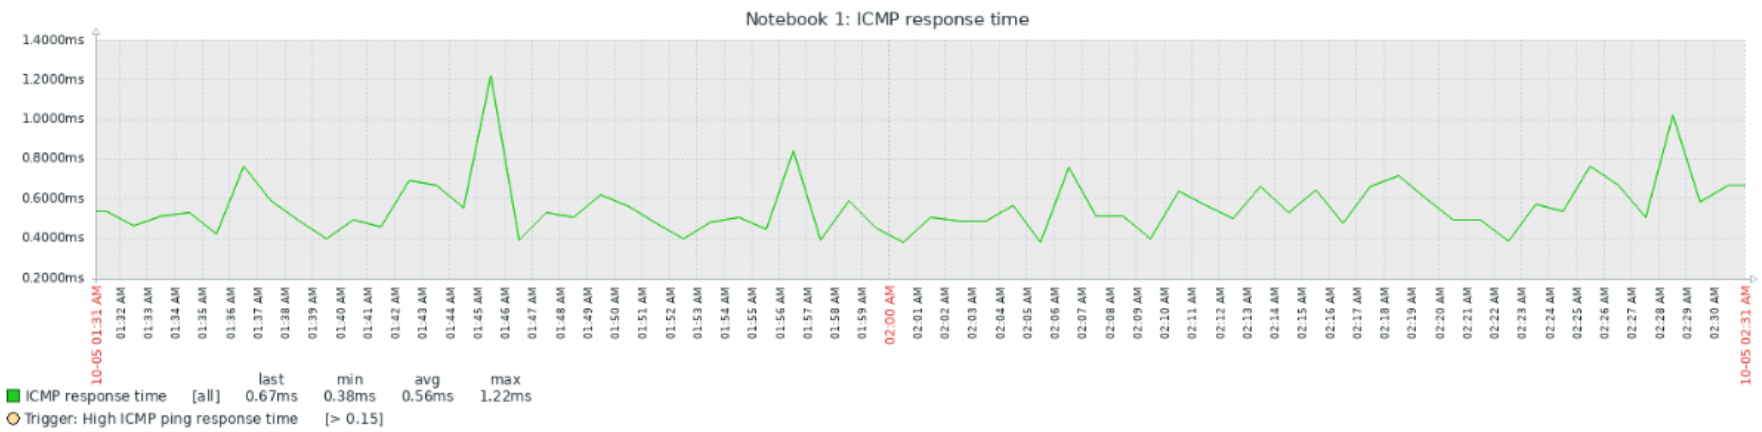
\includegraphics[width=0.9\linewidth]{Laptop_1.png}
  \caption{Tempo de resposta (ping) – Laptop 1}
  \label{fig:laptop_1_ping}
\end{figure}

O gráfico da Figura~\ref{fig:laptop_1_ping} demonstra que, apesar de haver variação nos tempos de resposta, o dispositivo respondeu consistentemente às requisições. Isso ocorre pois o \textit{Notebook 1} foi utilizado como hospedeiro da máquina virtual que executa o \textit{Zabbix Appliance}, além de atuar como dispositivo monitorado. O equipamento permaneceu ligado e em uso contínuo durante o intervalo das medições.

\subsection{Notebook 2}

\begin{figure}[h!]
  \centering
  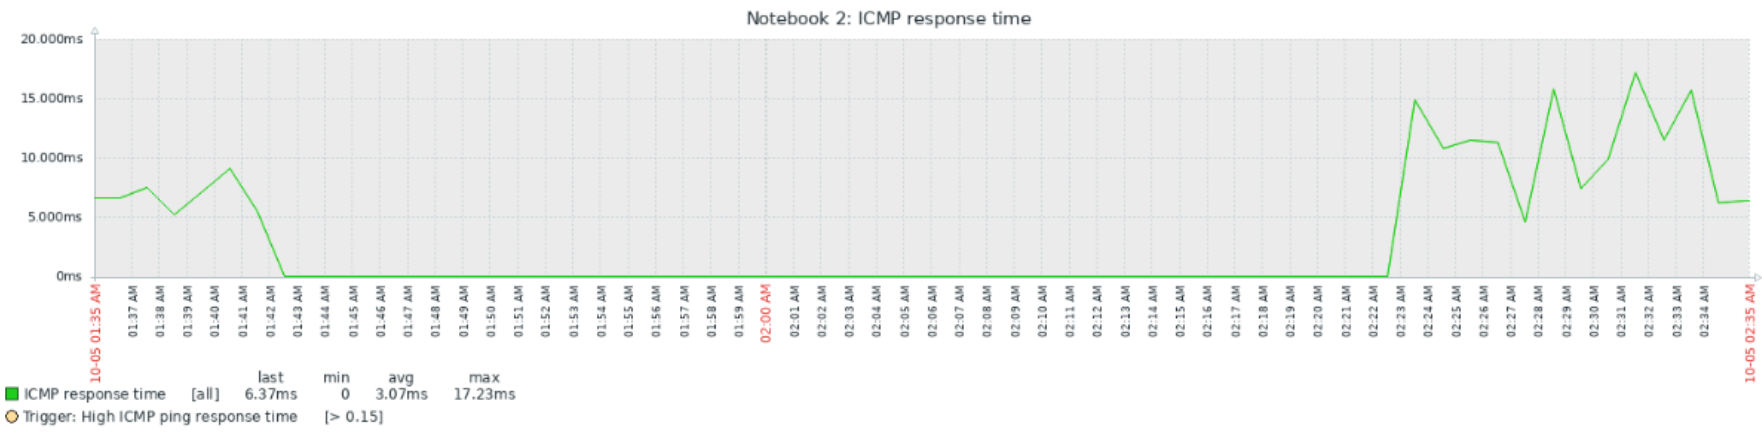
\includegraphics[width=0.9\linewidth]{Laptop_2.png}
  \caption{Tempo de resposta (ping) – Laptop 2}
  \label{fig:laptop_2_ping}
\end{figure}

Como pode ser observado na Figura~\ref{fig:laptop_2_ping}, há um intervalo em que não houve resposta às requisições ICMP. Isso se deve ao fato de o dispositivo estar operando com energia de bateria, não sendo utilizado ativamente. Nesse estado, entrou em modo de hibernação, o que impossibilitou a comunicação via \textit{ping} nesse período.

\subsection{Smartphone}

\begin{figure}[h!]
  \centering
  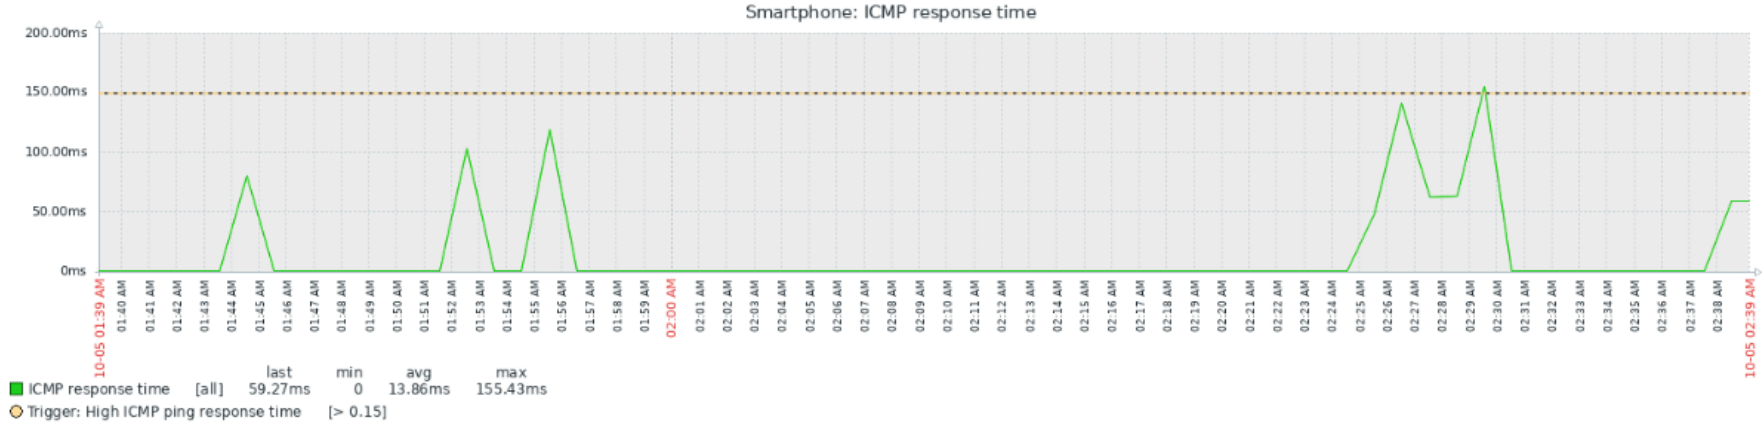
\includegraphics[width=0.9\linewidth]{Smartphone.png}
  \caption{Tempo de resposta (ping) – Smartphone}
  \label{fig:smartphone_ping}
\end{figure}

Conforme indicado na Figura~\ref{fig:smartphone_ping}, o smartphone não respondeu às requisições ICMP durante grande parte da medição. Diferentemente do \textit{Notebook 2}, o dispositivo não entra em modo de hibernação. Entretanto, fatores como a arquitetura do dispositivo e particularidades do sistema operacional móvel podem ter impedido as respostas ao \textit{ping}, resultando em longos períodos sem dados no gráfico.

% \subsection{Visualizando os testes no \textit{Wireshark}}
% \paragraph{}
% Paragraph

\section{Resultados de satisfação e desempenho da rede}
\paragraph{}
O questionário adotado para este trabalho foi o mesmo apresentado no curso de Administração e Gerência de Redes. O
questionário foi respondido por cinco usuários da rede:

\subsection{Desempenho da rede/Estabilidade da rede}

\noindent
\begin{minipage}{0.48\textwidth}
\centering
\begin{tikzpicture}
\begin{axis}[
    title={Desempenho da rede},
    ybar,
    bar width=15pt,
    enlargelimits=0.15,
    symbolic x coords={Ruim, Regular, Bom, Ótimo},
    xtick=data,
    nodes near coords,
    ymin=0,
]
\addplot coordinates {(Ruim, 1) (Regular, 2) (Bom, 1) (Ótimo, 1)};
\end{axis}
\end{tikzpicture}
\end{minipage}
\hfill
\begin{minipage}{0.48\textwidth}
\centering
\begin{tikzpicture}
\begin{axis}[
    title={Estabilidade da rede},
    ybar,
    bar width=15pt,
    enlargelimits=0.15,
    symbolic x coords={Ruim, Regular, Bom},
    xtick=data,
    nodes near coords,
    ymin=0,
]
\addplot coordinates {(Ruim, 2) (Regular, 2) (Bom, 1)};
\end{axis}
\end{tikzpicture}
\end{minipage}

\subsection{Qualidade do suporte técnico/Tempo de resposta do suporte técnico}

\noindent
\begin{minipage}{0.48\textwidth}
\centering
\begin{tikzpicture}
\begin{axis}[
    title={Qualidade do suporte técnico},
    ybar,
    bar width=15pt,
    enlargelimits=0.15,
    symbolic x coords={Ruim, Regular, Bom, Ótimo},
    xtick=data,
    nodes near coords,
    ymin=0,
]
\addplot coordinates {(Ruim, 1) (Regular, 1) (Bom, 2) (Ótimo, 1)};
\end{axis}
\end{tikzpicture}
\end{minipage}
\hfill
\begin{minipage}{0.48\textwidth}
\centering
\begin{tikzpicture}
\begin{axis}[
    title={Tempo de resposta do suporte},
    ybar,
    bar width=15pt,
    enlargelimits=0.15,
    symbolic x coords={Ruim, Regular},
    xtick=data,
    nodes near coords,
    ymin=0,
]
\addplot coordinates {(Ruim, 1) (Regular, 3)};
\end{axis}
\end{tikzpicture}
\end{minipage}

\subsection{Qualidade de acesso à rede externa/ Qualidade dos serviços prestados}

\noindent
\begin{minipage}{0.48\textwidth}
\centering
\begin{tikzpicture}
\begin{axis}[
    title={Qualidade do acesso à rede externa (Internet)},
    ybar,
    bar width=15pt,
    enlargelimits=0.15,
    symbolic x coords={Ruim, Regular},
    xtick=data,
    nodes near coords,
    ymin=0,
]
\addplot coordinates {(Ruim, 3) (Regular, 2)};
\end{axis}
\end{tikzpicture}
\end{minipage}
\hfill
\begin{minipage}{0.48\textwidth}
\centering
\begin{tikzpicture}
\begin{axis}[
    title={Qualidade dos serviços prestados},
    ybar,
    bar width=15pt,
    enlargelimits=0.15,
    symbolic x coords={Ruim, Regular, Bom},
    xtick=data,
    nodes near coords,
    ymin=0,
]
\addplot coordinates {(Ruim, 1) (Regular, 3) (Bom, 1)};
\end{axis}
\end{tikzpicture}
\end{minipage}

\subsection{Segurança de rede}

\begin{tikzpicture}
\begin{axis}[
    title={Segurança da rede},
    ybar,
    bar width=15pt,
    enlargelimits=0.15,
    symbolic x coords={Ruim, Regular},
    xtick=data,
    nodes near coords,
    ymin=0,
]
\addplot coordinates {(Ruim, 4) (Regular, 1)};
\end{axis}
\end{tikzpicture}

\section{SLA --- Acordo de Nível de Serviço}
\paragraph{}
O SLA foi elaborado em inglês. À seguir, o conteúdo do texto; também, pode ser consultado o código XML referente ao
contrato e ao \textit{schema} na seção de \nameref{sec:anexos}, sob ``\nameref{sec:contract}'' e ``\nameref{sec:schema}'',
respectivamente.

\subsection{Overview}
\subsubsection*{Clause 1}
This contract aims to establish a Service Level Agreement between the provider and the client. All clauses must be followed and respected. In case of non-compliance, both parties are subject to penalties.

\subsubsection*{Clause 2}
This contract is valid for 24 months from the effective start date defined at the end of the agreement.

\subsubsection*{Clause 3}
This agreement defines the services to be provided by the provider, including the required performance metrics that must be respected to maintain the quality level expected by the client. In case of breach, penalties are foreseen.

\subsection{Executive Summary}
\subsubsection*{Clause 4}
The responsibility for providing network management and administration services lies with the service provider, hereinafter referred to as "provider".

\subsubsection*{Clause 5}
The client will be referred to as "client" throughout this document.

\subsubsection*{Clause 6}
This Service Level Agreement aims to ensure the commitments and elements defined in this contract are delivered to the client by the provider. The services covered by this agreement include:
\begin{itemize}
  \item Security
  \item Availability of network resources
  \item Network resource administration and management
  \item Transparency
  \item Technical support and maintenance
\end{itemize}

\subsubsection*{Clause 7}
Network Operations Center (NOC) operating hours:
\begin{itemize}
  \item From 7:00 to 23:00 on business days
  \item From 8:00 to 20:00 on weekends and holidays
  \item Contact options:
  \begin{itemize}
    \item Phone: +00 (00) 0000-0000
    \item Email: support@sla-provider.com
  \end{itemize}
\end{itemize}

\subsubsection*{Clause 8}
In the event of emergency repairs (defined as high priority), the provider is required to respond within 12 hours from the time of the incident report. Non-compliance with this clause will result in a penalty of 5,500 DOL.

\subsubsection*{Clause 9}
The provider must notify the client via registered email about all scheduled maintenance operations that may cause service unavailability or impact.

\subsubsection*{Clause 10}
Monthly Reports – The provider must conduct monthly measurements and send availability reports to the client. Reports must include:
\begin{itemize}
  \item Resource availability statistics
  \item Statistics of resources allocated to the client, if any
  \item Scheduled maintenance for the month
\end{itemize}

\subsection{Performance Parameters and Metrics}
\subsubsection*{Clause 11}
A maintenance and repair window of 3 hours is reserved during low-traffic periods with prior notice to the client.

\subsubsection*{Clause 12}
External network access must maintain 100\% availability. The data processing center responsible for routing to the internet backbone must be available at all times via the main route or alternate links.

\subsection{Scope of Service}
\subsubsection*{Clause 13}
The following items and thresholds must be respected:
\begin{itemize}
  \item The number of threads on workstations must not exceed 2000
  \item The network interface of the workstation host must always be operational
  \item The management host must not have zero uptime during the monitoring period
  \item The number of available inodes must not drop below 90\%
  \item The number of active connections on port 443 of the Notebook host must not exceed 10
\end{itemize}

\subsection{Penalties}
\subsubsection*{Clause 14}
This clause defines the penalties applied to the provider in case of breach:
\begin{itemize}
  \item For any breach of clause, the responsible party must pay a fine of 1,500 DOL to the affected party
  \item For non-compliance with Item 2 of Clause 13, the provider must pay 15,000 DOL to the client
  \item For breach of two or more clauses, the client has the right to review the contract. If more than 12 months have passed since the contract start date, the client may request termination
\end{itemize}

\subsection{Mutual Responsibilities}
\subsubsection*{Clause 15}
This agreement is valid from the effective date defined below. Upon contract termination or after 12 months, a revision by both parties is required.

\subsubsection*{Clause 16}
Contract revision shall be conducted in a meeting where both parties decide whether to renew the agreement for the next period. After the decision, both parties have 30 days to formally submit clause changes.

\subsubsection*{Clause 17}
The provider is responsible for fulfilling all services and guarantees defined in this agreement, covering the defined hours and respecting the established metrics.

\subsubsection*{Clause 18}
The client is responsible for complying with the terms of this agreement, respecting service coverage hours, and providing required information resulting from the service usage. The client is also responsible for the monthly payment of 2,000 DOL to the provider.

\newpage
\section{Anexos}\label{sec:anexos}
\subsection{Configuração do \textit{Zabbix}/Docker-compose}\label{sec:yaml}
\texttt{docker-compose.yaml}
\begin{lstlisting}
version: '3.5'
services:
  zabbix-server:
    container\_name: "zabbix-server"
    image: zabbix/zabbix-server-pgsql:alpine-trunk
    restart: always
    ports:
      - 10051:10051
    networks:
      - zabbix7
    volumes:
      - /etc/localtime:/etc/localtime:ro
      - /etc/timezone:/etc/timezone:ro 
    environment:
      ZBX\_CACHESIZE: 4096M
      ZBX\_HISTORYCACHESIZE: 1024M
      ZBX\_HISTORYINDEXCACHESIZE: 1024M
      ZBX\_TRENDCACHESIZE: 1024M
      ZBX\_VALUECACHESIZE: 1024M
      DB\_SERVER\_HOST: "192.168.0.19" 
      DB\_PORT: 5432
      POSTGRES\_USER: "zabbix"
      POSTGRES\_PASSWORD: "zabbix"
      POSTGRES\_DB: "zabbix\_db"
    stop\_grace\_period: 30s
    labels:
      com.zabbix.description: "Zabbix server with PostgreSQL database support"
      com.zabbix.company: "Zabbix LLC"
      com.zabbix.component: "zabbix-server"
      com.zabbix.dbtype: "pgsql"
      com.zabbix.os: "alpine"

  zabbix-web-nginx-pgsql:
    container\_name: "zabbix-web"
    image: zabbix/zabbix-web-nginx-pgsql:alpine-trunk
    restart: always
    ports:
      - 8080:8080
      - 8443:8443
    volumes:
      - /etc/localtime:/etc/localtime:ro
      - /etc/timezone:/etc/timezone:ro
      - ./cert/:/usr/share/zabbix/conf/certs/:ro
    networks:
      - zabbix7
    environment:
      DB\_SERVER\_HOST: "192.168.0.19"
      DB\_PORT: 5432
      POSTGRES\_USER: "zabbix"
      POSTGRES\_PASSWORD: "zabbix"
      POSTGRES\_DB: "zabbix\_db"
      ZBX\_MEMORYLIMIT: "1024M"
    depends\_on:
      - zabbix-server
    healthcheck:
      test: ["CMD", "curl", "-f", "http://localhost:8080/ping"]
      interval: 10s
      timeout: 5s
      retries: 3
      start\_period: 30s
    stop\_grace\_period: 10s
    labels:
      com.zabbix.description: "Zabbix frontend on Nginx web-server with PostgreSQL database support"
      com.zabbix.company: "Zabbix LLC"
      com.zabbix.component: "zabbix-frontend"
      com.zabbix.webserver: "nginx"
      com.zabbix.dbtype: "pgsql"
      com.zabbix.os: "alpine"

  zabbix-db-agent2:
    container\_name: "zabbix-agent2"
    image: zabbix/zabbix-agent2:alpine-trunk
    user: root
    depends\_on:
      - zabbix-server
    volumes:
      - /etc/localtime:/etc/localtime:ro
      - /etc/timezone:/etc/timezone:ro
      - /run/docker.sock:/var/run/docker.sock
    environment:
      ZBX\_HOSTNAME: "zabbix7"
      ZBX\_SERVER\_HOST: "127.0.0.1"
      ZBX\_PASSIVE\_ALLOW: "true"
      ZBX\_PASSIVESERVERS: "192.168.0.19"
      ZBX\_ENABLEREMOTECOMMANDS: "1"
      ZBX\_ACTIVE\_ALLOW: "false"
      ZBX\_DEBUGLEVEL: "3"
    privileged: true
    pid: "host"
    ports:
      - 10050:10050
      - 31999:31999 
    networks:
      - zabbix7
    stop\_grace\_period: 5s
   
  db:
    container\_name: "zabbix\_db"
    image: postgres:15.6-bullseye
    restart: always
    volumes:
     - zbx\_db15:/var/lib/postgresql/data
    ports:
     - 5432:5432
    networks:
     - zabbix7
    environment:
     POSTGRES\_USER: "zabbix"
     POSTGRES\_PASSWORD: "zabbix"
     POSTGRES\_DB: "zabbix\_db"

networks:
  zabbix7:
   driver: bridge
volumes:
  zbx\_db15:
\end{lstlisting}

\subsection{Contrato SLA}\label{sec:contract}

\texttt{contract.xml}
\begin{lstlisting}
<?xml version="1.0" encoding="UTF-8" standalone="yes"?>
<sla>
  <title>SERVICE LEVEL AGREEMENT CONTRACT</title>
  <section>
    6.1 Overview
    <clause>
      Clause 1.
      <description>
        This contract aims to establish a Service Level Agreement between the provider and the client. All clauses must be followed and respected. In case of non-compliance, both parties are subject to penalties.
      </description>
    </clause>
    <clause>
      Clause 2.
      <description>
        This contract is valid for 24 months from the effective start date defined at the end of the agreement.
      </description>
    </clause>
    <clause>
      Clause 3.
      <description>
        This agreement defines the services to be provided by the provider, including the required performance metrics that must be respected to maintain the quality level expected by the client. In case of breach, penalties are foreseen.
      </description>
    </clause>
  </section>
  <section>
    6.2 Executive Summary
    <clause>
      Clause 4.
      <description>
        The responsibility for providing network management and administration services lies with the service provider, hereinafter referred to as "provider".
      </description>
    </clause>
    <clause>
      Clause 5.
      <description>
        The client will be referred to as "client" throughout this document.
      </description>
    </clause>
    <clause>
      Clause 6.
      <description>
        This Service Level Agreement aims to ensure the commitments and elements defined in this contract are delivered to the client by the provider. The services covered by this agreement include:
        <description_item>Security</description_item>
        <description_item>Availability of network resources</description_item>
        <description_item>Network resource administration and management</description_item>
        <description_item>Transparency</description_item>
        <description_item>Technical support and maintenance</description_item>
      </description>
    </clause>
    <clause>
      Clause 7.
      <description>
        Network Operations Center (NOC) operating hours:
        <description_item>From 7:00 to 23:00 on business days</description_item>
        <description_item>From 8:00 to 20:00 on weekends and holidays</description_item>
        The support team may be contacted through:
        <description_item>Phone: +00 (00) 0000-0000</description_item>
        <description_item>Email: support@sla-provider.com</description_item>
      </description>
    </clause>
    <clause>
      Clause 8.
      <description>
        In the event of emergency repairs (defined as high priority), the provider is required to respond within 12 hours from the time of the incident report. Non-compliance with this clause will result in a penalty of 5,500 DOL.
      </description>
    </clause>
    <clause>
      Clause 9.
      <description>
        The provider must notify the client via registered email about all scheduled maintenance operations that may cause service unavailability or impact.
      </description>
    </clause>
    <clause>
      Clause 10.
      <description>
        Monthly Reports – The provider must conduct monthly measurements and send availability reports to the client. Reports must include:
        <description_item>Resource availability statistics</description_item>
        <description_item>Statistics of resources allocated to the client, if any</description_item>
        <description_item>Scheduled maintenance for the month</description_item>
      </description>
    </clause>
  </section>
  <section>
    6.3 Performance Parameters and Metrics
    <clause>
      Clause 11.
      <description>
        A maintenance and repair window of 3 hours is reserved during low-traffic periods with prior notice to the client.
      </description>
    </clause>
    <clause>
      Clause 12.
      <description>
        External network access must maintain 100% availability. The data processing center responsible for routing to the internet backbone must be available at all times via the main route or alternate links.
      </description>
    </clause>
  </section>
  <section>
    6.4 Scope of Service
    <clause>
      Clause 13.
      <description>
        The following items and thresholds must be respected:
        <description_item>The number of threads on workstations must not exceed 2000</description_item>
        <description_item>The network interface of the workstation host must always be operational</description_item>
        <description_item>The management host must not have zero uptime during the monitoring period</description_item>
        <description_item>The number of available inodes must not drop below 90%</description_item>
        <description_item>The number of active connections on port 443 of the Notebook host must not exceed 10</description_item>
      </description>
    </clause>
  </section>
  <section>
    6.5 Penalties
    <clause>
      Clause 14.
      <description>
        This clause defines the penalties applied to the provider in case of breach:
        <description_item>For any breach of clause, the responsible party must pay a fine of 1,500 DOL to the affected party</description_item>
        <description_item>For non-compliance with Item 2 of Clause 13, the provider must pay 15,000 DOL to the client</description_item>
        <description_item>For breach of two or more clauses, the client has the right to review the contract. If more than 12 months have passed since the contract start date, the client may request termination</description_item>
      </description>
    </clause>
  </section>
  <section>
    6.6 Mutual Responsibilities
    <clause>
      Clause 15.
      <description>
        This agreement is valid from the effective date defined below. Upon contract termination or after 12 months, a revision by both parties is required.
      </description>
    </clause>
    <clause>
      Clause 16.
      <description>
        Contract revision shall be conducted in a meeting where both parties decide whether to renew the agreement for the next period. After the decision, both parties have 30 days to formally submit clause changes.
      </description>
    </clause>
    <clause>
      Clause 17.
      <description>
        The provider is responsible for fulfilling all services and guarantees defined in this agreement, covering the defined hours and respecting the established metrics.
      </description>
    </clause>
    <clause>
      Clause 18.
      <description>
        The client is responsible for complying with the terms of this agreement, respecting service coverage hours, and providing required information resulting from the service usage. The client is also responsible for the monthly payment of 2,000 DOL to the provider.
      </description>
    </clause>
  </section>
</sla>
\end{lstlisting}

\subsection{Schema de validação XML para contrato}\label{sec:schema}

\texttt{schema.xml}
\begin{lstlisting}
<xs:schema attributeFormDefault="unqualified" elementFormDefault="qualified" xmlns:xs="http://www.w3.org/2001/XMLSchema">
  <xs:element name="sla">
    <xs:complexType>
       <xs:sequence>
        <xs:element type="xs:string" name="title"/>
        <xs:element name="section" maxOccurs="unbounded" minOccurs="0"> 
          <xs:complexType mixed="true">
            <xs:sequence>
              <xs:element name="clause" maxOccurs="unbounded" minOccurs="0">
                <xs:complexType mixed="true">
                  <xs:sequence>
                    <xs:element name="description">
                      <xs:complexType mixed="true">
                        <xs:sequence>
                          <xs:element type="xs:string" name="description_item" maxOccurs="unbounded" minOccurs="0"/>
                        </xs:sequence>
                      </xs:complexType>
                    </xs:element>
                  </xs:sequence>
                </xs:complexType>
              </xs:element>
            </xs:sequence>
          </xs:complexType>
        </xs:element>
        <xs:element name="signatures"> </xs:element>
      </xs:sequence>
    </xs:complexType>
  </xs:element>
</xs:schema>
\end{lstlisting}
\newpage

\bibliographystyle{ieeetr}
\bibliography{references}

\end{document}
